\documentclass{beamer}
\usepackage{HECbeamer}
% \usepackage{pgfpages}
% \pgfpagesuselayout{4 on 1}[letterpaper, landscape, border shrink=5mm]
\title[\color{white}{MATH 60604A \S~5a - Correlated data}]{\texorpdfstring{MATH 60604A \\Statistical modelling \\ \S~5a - Correlated data}{MATH 60604A \\Statistical modelling \\ \S~5a - Correlated data}}
\author{Léo Belzile}
\institute{HEC Montréal\\
Department of Decision Sciences}
\date{} 

\begin{document}
\frame{\titlepage}
\begin{frame}
\frametitle{Modifications of the ordinary linear regression model}
\bi \item The goal of this chapter is to show how the linear regression model can be modified to account for the dependence between observations.
\item 
We focus on modelling the covariance matrix to account for dependence between observations (for longitudinal data and clustered data) and heteroscedasticity (different variance per group).
\ei

\end{frame}
\begin{frame}
 \frametitle{When independence fails}
 \begin{itemize}
  \item When observations are positively correlated, the estimated standard errors of the coefficients of the linear model are \textbf{too small}.
  \item We are overconfident and will reject the null hypothesis more often then we should if the null is true (inflated Type I error, false positives).
  
  \end{itemize}
  \end{frame}
  \begin{frame}
  \frametitle{Sources of correlation}
  Generally, correlation between observations can come from 
\bi
\item  time dependence, roughly categorized into
\bi \item longitudinal data: repeated measurements are taken from the same subjects (few time points)
\item time series: observations observed at multiple time periods (many time points). Time series require dedicated models not covered in this course.
\ei 
\item  clustered data: measurements are taken from subjects that are not independent from one another (family, groups, etc.)
\ei
\end{frame}


\begin{frame}
\frametitle{Moments of random vectors}
\bi
% \item As we'll see how to fit the regression model to account for correlation between observations and unequal variance, it's important to understand correlation structures.
\item Consider a \alert{random vector} $\bs{Y}$ of dimension $n$. 
\bi
\item Such a vector would usually comprise
repeated measures on an individual, or even observations from a group of individuals. 
\ei
\item The expected value (theoretical mean) of this vector $\E{\bs{Y}}$ is taken componentwise, i.e., $\E{\bs{Y}} = (\E{Y_1}, \ldots, \E{Y_n})$.
\item We denote the variance of the $i$th component by $\sigma_{ii} = \sigma^2_i=\Va{Y_i}$.
\item Similarly, the covariance between observations $Y_i$ and $Y_j$ is  $\sigma_{ij}=\Co{Y_i, Y_j}$.
\ei
\end{frame}

\begin{frame}
\frametitle{Covariance matrix}
\bi
\item For a random vector $\bs{Y}$, 
we define the \alert{covariance matrix} as the  $n\times n$ symmetric matrix
\[
\Co{\bs{Y}}=
  \begin{pmatrix}
    \sigma_1^2 & \sigma_{12} & \sigma_{13} & \cdots & \sigma_{1n} \\
     \sigma_{21} & \sigma_{2}^2 & \sigma_{23} & \cdots & \sigma_{2n} \\
      \sigma_{31} & \sigma_{32} & \sigma_{3}^2 & \ddots & \sigma_{3n} \\
    \vdots &  \vdots &  \ddots & \ddots &  \vdots \\
        \sigma_{n1} & \sigma_{n2} & \sigma_{n3} & \cdots & \sigma_{n}^2 \\
  \end{pmatrix}.
\]
\item The $i$th diagonal element of $\Co{\bs{Y}}$ is the variance of $Y_i$.
\item Since the matrix is symmetric, $\sigma_{ij}=\sigma_{ji}$.
\ei
\end{frame}

\begin{frame}
\frametitle{Covariance and correlation matrix}
\bi
\item The correlation between $Y_i$ and $Y_j$ is 
\begin{align*}
\rho_{ij}=\Cor{Y_i, Y_j}=\frac{\sigma_{ij}}{\sigma_i\sigma_j}.
\end{align*}
\item The \alert{correlation matrix} of $\bs{Y}$ is an
$n\times n$ symmetric matrix with ones on the diagonal and the pairwise correlations off the diagonal, 
\[
\Cor{\bs{Y}}=
  \begin{pmatrix}
    1 & \rho_{12} & \rho_{13} & \cdots & \rho_{1n} \\
     \rho_{21} & 1 & \rho_{23}& \cdots & \rho_{2n} \\
     \rho_{31} & \rho_{32} & 1& \ddots & \rho_{3n} \\
    \vdots &  \vdots &  \ddots & \ddots &  \vdots \\
        \rho_{n1} & \rho_{n2} & \rho_{n3} & \cdots & 1 \\
  \end{pmatrix}.
\]
\ei
\end{frame}
\begin{frame}
\frametitle{Modelling correlation/covariance between measurements}
 One of the most important parts of modelling 
correlated (or longitudinal) data is the need to account for within-group correlations. 
\bi \item This basically comes down to modelling a covariance matrix for observations within the same group (or within the same individual in the case of repeated measures).
\ei
\end{frame}


\begin{frame}[fragile]
\frametitle{Longitudinal studies on independent subjects}
\bi
\item In this kind of study, several measurements are taken from the same individuals, usually over time. 
\bi

\item these data are termed \alert{repeated measures} or \alert{longitudinal data}, but econometricians use the vocable \alert{panel data}. 
\ei
\item The individuals are \alert{independent} from one another; however, measurements from the same subject are not independent.
\item A data file might look like 
{\footnotesize 
\begin{table}
\centering

\begin{tabular}{cccc}
 \toprule 
 \textbf{subject} & \textbf{time} & \textbf{score} & \textbf{sex}\\
 \midrule 
 1 & 1 & 5 & 0 \\
 1 & 2 & 6 & 0 \\
 1 & 3 & 4 & 0 \\
 2 & 1 & 2 & 1 \\
 2 & 2 & 4 & 1 \\
 2 & 3 & 7 & 1 \\
 \bottomrule
\end{tabular}
\end{table}
}


% \begin{center}
% \includegraphics[scale=0.25]{Figures/exemple.png}
% \end{center}
\ei
\end{frame}

\begin{frame}
\frametitle{Studies on subjects that are not independent}
\bi
\item In this kind of study, the subjects are sampled within a \alert{group}.
\item Here are several examples:
\bi

\item subjects sampled from the same household,
\item subjects sampled from within several businesses,
\item subjects sampled within schools, hospitals, etc. 
\ei
\item In all these examples, the measurements between subjects in the same group (household, school, business) are correlated.
\ei
\end{frame}

\begin{frame}
\frametitle{Correlated data \textbf{is} grouped data}
\bi
\item We can always consider correlated data as grouped data, where there is within-group correlation.
\item In longitudinal data, we have several records for each individual.
\item In other examples, the groups could be households, schools, hospitals, businesses, etc.
\ei
\begin{center}
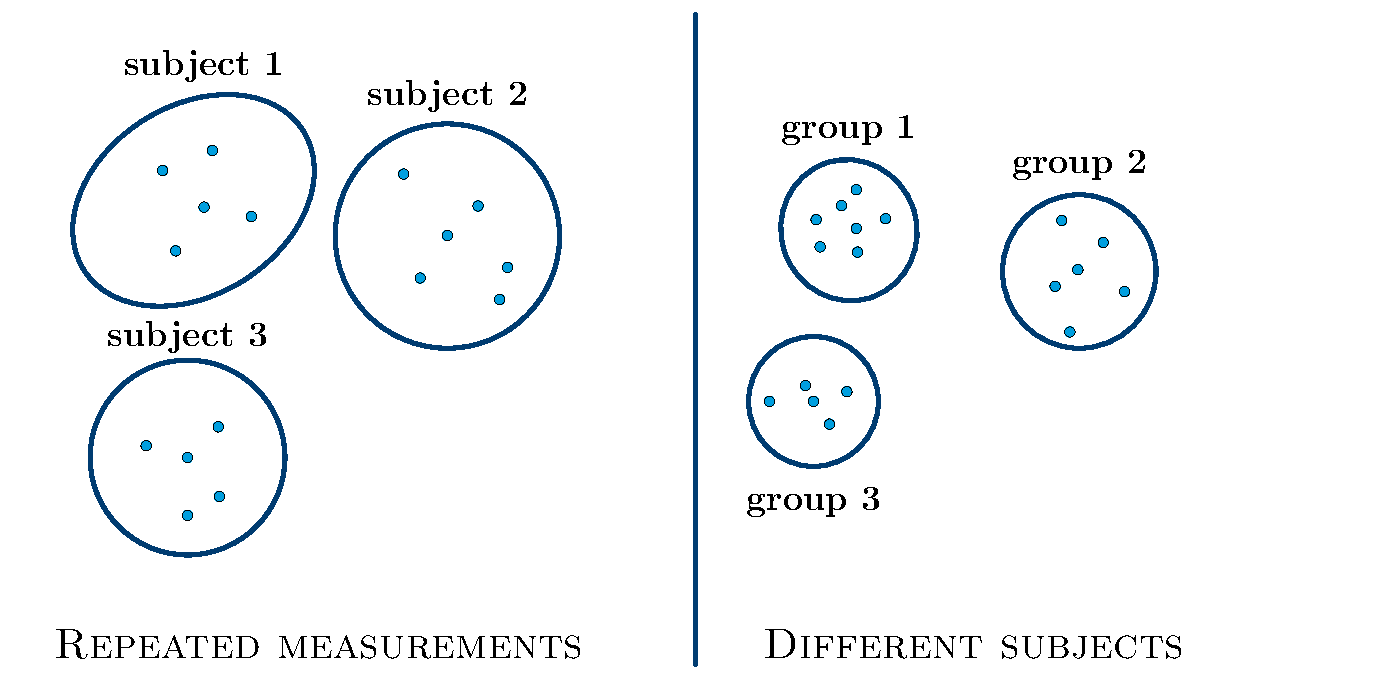
\includegraphics[width = 0.8\linewidth]{img/c5/06-correlated-groups.pdf}
\end{center}
One dot equals one line in the data file.
\end{frame} 


\begin{frame}
\frametitle{What happens if we ignore within-group correlation?}
\bi
\item Suppose that we have grouped data and we perform a one-sample $t$-test with level $\alpha=5\%$.
\item The following figure shows the true Type I error probability as a function of the within-group correlation for different values of the group size $m$. 
\begin{center}
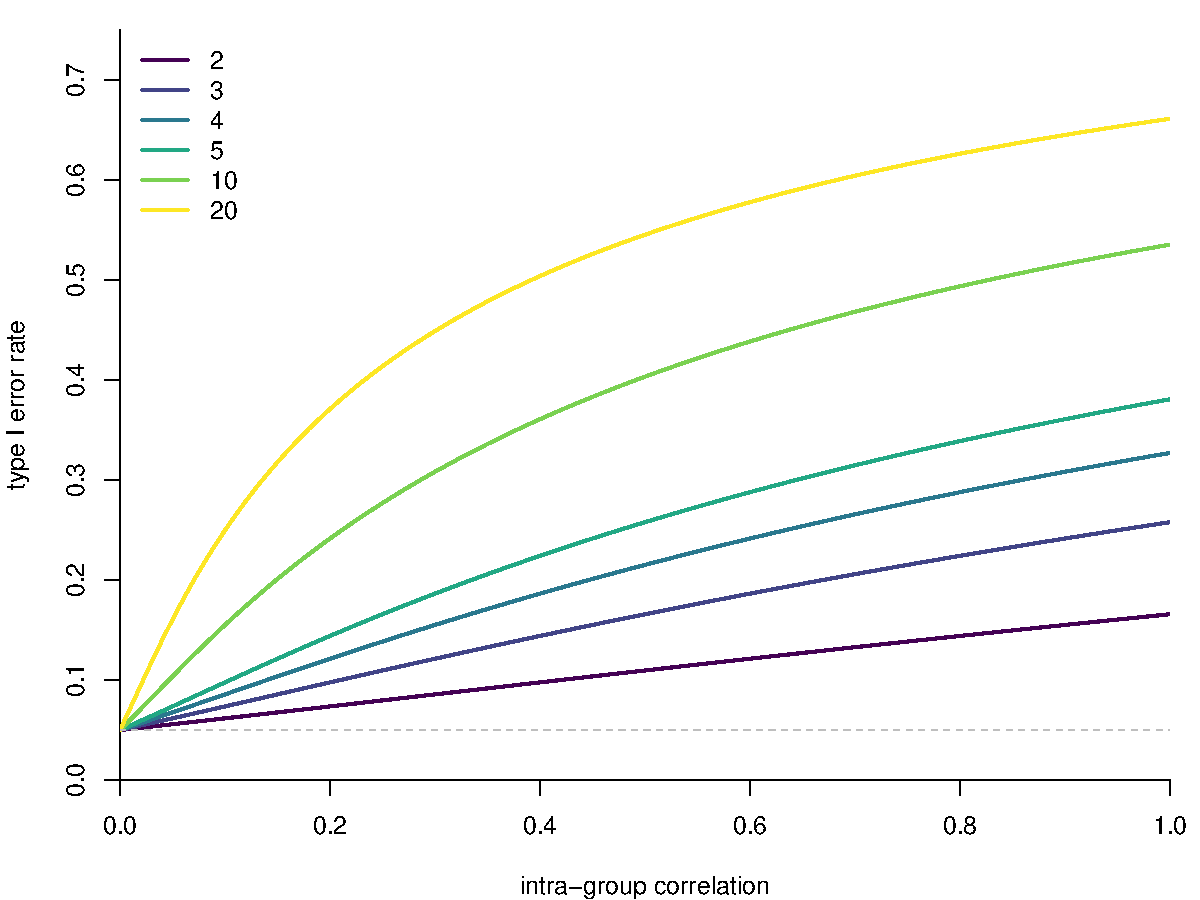
\includegraphics[width = 0.65 \linewidth]{img/c5/06-correlated-typeIerrorinf.pdf}
\end{center}
\ei
\end{frame}
 



\begin{frame}
\frametitle{Type I error inflation with correlated data}
\bi
\item It is alarming to see how quickly the probability of a Type I error increases with correlation, as well as with the number of samples within each group. 
\item The conclusions drawn from the $t$-tests are invalid, since they do not account for the within-group correlation.
\item The size distortion illustrates the fact that \alert{statistical inference is typically no longer valid}
when we use a method that assumes independence between observations, when in truth the data are correlated.
\ei
\end{frame}

\end{document}
